\section{Introduction}

Ce chapitre présente la modélisation et l'implémentation de notre solution de gestion de projets. Nous y détaillerons d'abord les blocs fonctionnels qui constituent le cœur de la plateforme, puis nous présenterons les diagrammes de modélisation qui illustrent l'architecture et les interactions du système.

\section{Blocs fonctionnels de la solution}

Cette section détaille les fonctionnalités clés et les capacités de la plateforme de gestion de projets, démontrant comment elle répond aux besoins des différents rôles utilisateurs et couvre l'ensemble du cycle de vie d'un projet (projets, phases, sprints, user stories, tâches, livrables, validations, changements, ressources, affectations, notifications, rapports).

\section{Bloc fonctionnel : Gestion des Utilisateurs et Authentification}

\subsection{1.1. Authentification Utilisateur}
\textbf{Description :} Permettre aux utilisateurs de se connecter au système via authentification locale ou OAuth2 Microsoft.
\textbf{Entrée(s) :} Email/identifiant et mot de passe, ou bouton OAuth2 Microsoft.
\textbf{Sortie(s) :} Jeton JWT valide et redirection vers le tableau de bord.
\textbf{Importance de réalisation :} Haute

\subsection{1.2. Gestion des Rôles et Permissions}
\textbf{Description :} Attribuer et gérer les rôles utilisateurs (ADMIN, MANAGER, DÉVELOPPEUR, PRODUCT\_OWNER, SCRUM\_MASTER, etc.).
\textbf{Entrée(s) :} Sélection de rôles système et rôles projet par utilisateur.
\textbf{Sortie(s) :} Permissions d'accès configurées et contrôlées.
\textbf{Importance de réalisation :} Haute

\subsection{1.3. Gestion du Profil Utilisateur}
\textbf{Description :} Consulter et modifier les informations personnelles et préférences de notification.
\textbf{Entrée(s) :} Champs éditables (nom, email, téléphone, préférences).
\textbf{Sortie(s) :} Confirmation de mise à jour et profil actualisé.
\textbf{Importance de réalisation :} Moyenne

\subsection{1.4. Déconnexion Sécurisée}
\textbf{Description :} Fermer la session utilisateur et invalider les jetons d'authentification.
\textbf{Entrée(s) :} Bouton de déconnexion.
\textbf{Sortie(s) :} Session fermée et redirection vers la page de connexion.
\textbf{Importance de réalisation :} Haute

\begin{table}[H]
\centering
\footnotesize
\begin{tabular}{|p{1.5cm}|p{3.5cm}|p{1.5cm}|p{1.5cm}|p{2cm}|p{2.5cm}|}
\hline
\textbf{Règle} & \textbf{Description} & \textbf{Type} & \textbf{Priorité} & \textbf{Validation} & \textbf{Message d'erreur} \\
\hline
RG-AUTH-01 & L'email doit être unique dans le système & Référentiel & Haute & Backend + Frontend & «Email déjà utilisé» \\
\hline
RG-AUTH-02 & Les mots de passe doivent respecter la politique de sécurité & Sécurité & Haute & Frontend + Backend & «Mot de passe non conforme» \\
\hline
RG-AUTH-03 & Seul un administrateur peut créer des comptes utilisateur & Contrôle d'accès & Haute & Backend & «Création non autorisée» \\
\hline
RG-AUTH-04 & Les jetons JWT doivent être valides et non expirés & Sécurité & Haute & Backend & «Token invalide ou expiré» \\
\hline
RG-AUTH-05 & La déconnexion doit invalider tous les jetons actifs & Sécurité & Haute & Backend & «Déconnexion échouée» \\
\hline
\end{tabular}
\caption{Règles de gestion - Gestion des Utilisateurs et Authentification}
\label{tab:rg_auth}
\end{table}

\section{Bloc fonctionnel : Gestion des Projets}

\subsection{2.1. Création de Projet}
\textbf{Description :} Créer un nouveau projet avec ses paramètres de base et méthodologie.
\textbf{Entrée(s) :} Nom, type de méthodologie (SCRUM/Itératif), dates, budget, description, client associé.
\textbf{Sortie(s) :} Projet créé avec identifiant unique et état initial.
\textbf{Importance de réalisation :} Haute

\subsection{2.2. Gestion des Phases}
\textbf{Description :} Organiser le cycle de vie du projet en phases (Initialisation, Planification, Exécution, Maîtrise, Clôture).
\textbf{Entrée(s) :} Dates de début/fin par phase et tâches associées.
\textbf{Sortie(s) :} Planning structuré avec suivi d'avancement par phase.
\textbf{Importance de réalisation :} Haute

\subsection{2.3. Gestion du Backlog}
\textbf{Description :} Créer et maintenir le backlog produit avec versioning des exigences.
\textbf{Entrée(s) :} User stories, critères d'acceptation, priorités et versions.
\textbf{Sortie(s) :} Backlog versionné avec traçabilité des évolutions.
\textbf{Importance de réalisation :} Haute

\subsection{2.4. Gestion des Jalons}
\textbf{Description :} Définir et suivre les points de contrôle critiques du projet.
\textbf{Entrée(s) :} Date prévue, description du jalon et critères de validation.
\textbf{Sortie(s) :} Jalons avec statut d'atteinte et alertes de retard.
\textbf{Importance de réalisation :} Moyenne

\subsection{2.5. Gestion des Parties Prenantes}
\textbf{Description :} Centraliser les informations de contact et rôles des acteurs du projet.
\textbf{Entrée(s) :} Informations de contact, rôles et responsabilités.
\textbf{Sortie(s) :} Répertoire des parties prenantes avec rôles définis.
\textbf{Importance de réalisation :} Moyenne

\begin{table}[H]
\centering
\footnotesize
\begin{tabular}{|p{1.5cm}|p{3.5cm}|p{1.5cm}|p{1.5cm}|p{2cm}|p{2.5cm}|}
\hline
\textbf{Règle} & \textbf{Description} & \textbf{Type} & \textbf{Priorité} & \textbf{Validation} & \textbf{Message d'erreur} \\
\hline
RG-PROJ-01 & Un projet doit avoir un nom unique & Référentiel & Haute & Backend + Frontend & «Nom de projet déjà existant» \\
\hline
RG-PROJ-02 & Les dates de fin doivent être postérieures aux dates de début & Cohérence & Haute & Frontend + Backend & «Date de fin invalide» \\
\hline
RG-PROJ-03 & Le budget doit être positif & Cohérence & Haute & Frontend + Backend & «Budget invalide» \\
\hline
RG-PROJ-04 & Les phases doivent se succéder dans l'ordre logique & Cohérence & Haute & Backend & «Ordre des phases invalide» \\
\hline
RG-PROJ-05 & Les jalons doivent avoir des dates cohérentes avec les phases & Cohérence & Moyenne & Backend & «Date de jalon incohérente» \\
\hline
\end{tabular}
\caption{Règles de gestion - Gestion des Projets}
\label{tab:rg_projets}
\end{table}

\section{Bloc fonctionnel : Gestion Agile}

\subsection{3.1. Gestion des Sprints}
\textbf{Description :} Créer et planifier les sprints avec objectifs, dates et capacité d'équipe.
\textbf{Entrée(s) :} Objectifs du sprint, dates de début/fin, user stories sélectionnées.
\textbf{Sortie(s) :} Sprint planifié avec vélocité estimée et charge d'équipe.
\textbf{Importance de réalisation :} Haute

\subsection{3.2. Gestion des User Stories}
\textbf{Description :} Créer et gérer les user stories avec critères d'acceptation et priorités.
\textbf{Entrée(s) :} Titre, description, critères d'acceptation, priorité, estimation en points.
\textbf{Sortie(s) :} User story avec état de progression et rattachement au sprint.
\textbf{Importance de réalisation :} Haute

\subsection{3.3. Gestion des Tâches}
\textbf{Description :} Créer et assigner des tâches avec suivi d'état et gestion des obstacles.
\textbf{Entrée(s) :} Description, durée estimée, priorité, assignation utilisateur.
\textbf{Sortie(s) :} Tâche avec état de progression et suivi des obstacles.
\textbf{Importance de réalisation :} Haute

\subsection{3.4. Tableau Kanban}
\textbf{Description :} Visualiser et gérer les tâches et user stories par état avec glisser-déposer.
\textbf{Entrée(s) :} Filtres par projet, sprint, utilisateur, priorité.
\textbf{Sortie(s) :} Vue Kanban interactive avec colonnes configurables.
\textbf{Importance de réalisation :} Haute

\begin{table}[H]
\centering
\footnotesize
\begin{tabular}{|p{1.5cm}|p{3.5cm}|p{1.5cm}|p{1.5cm}|p{2cm}|p{2.5cm}|}
\hline
\textbf{Règle} & \textbf{Description} & \textbf{Type} & \textbf{Priorité} & \textbf{Validation} & \textbf{Message d'erreur} \\
\hline
RG-AGILE-01 & La date de fin d'un sprint doit être postérieure à sa date de début & Cohérence & Haute & Frontend + Backend & «Date de fin invalide» \\
\hline
RG-AGILE-02 & Une user story doit avoir au moins un critère d'acceptation & Cohérence & Haute & Frontend + Backend & «Critères d'acceptation manquants» \\
\hline
RG-AGILE-03 & Les tâches doivent être assignées à un utilisateur valide & Cohérence & Haute & Backend & «Utilisateur invalide» \\
\hline
RG-AGILE-04 & Les transitions d'état doivent respecter le workflow défini & Cohérence & Haute & Backend & «Transition d'état invalide» \\
\hline
RG-AGILE-05 & Les estimations doivent être des nombres entiers positifs & Cohérence & Moyenne & Frontend + Backend & «Estimation invalide» \\
\hline
\end{tabular}
\caption{Règles de gestion - Gestion Agile}
\label{tab:rg_agile}
\end{table}

\section{Bloc fonctionnel : Gestion des Ressources et Affectations}

\subsection{4.1. Gestion des Ressources}
\textbf{Description :} Gérer les ressources humaines, matérielles et financières du projet.
\textbf{Entrée(s) :} Type de ressource, disponibilité, compétences, contraintes d'utilisation.
\textbf{Sortie(s) :} Catalogue de ressources avec planification et optimisation des coûts.
\textbf{Importance de réalisation :} Haute

\subsection{4.2. Affectation des Rôles Projet}
\textbf{Description :} Attribuer des rôles spécifiques aux utilisateurs selon le contexte du projet.
\textbf{Entrée(s) :} Sélection utilisateur et rôle projet (MOA, MOE, PO, SM, DEV, etc.).
\textbf{Sortie(s) :} Affectations avec permissions d'accès et responsabilités définies.
\textbf{Importance de réalisation :} Haute

\subsection{4.3. Gestion d'Équipe}
\textbf{Description :} Constituer et organiser les équipes projet avec recherche de compétences.
\textbf{Entrée(s) :} Critères de recherche (compétences, disponibilité, charge de travail).
\textbf{Sortie(s) :} Équipe constituée avec planification des charges et suivi de disponibilité.
\textbf{Importance de réalisation :} Moyenne

\begin{table}[H]
\centering
\footnotesize
\begin{tabular}{|p{1.5cm}|p{3.5cm}|p{1.5cm}|p{1.5cm}|p{2cm}|p{2.5cm}|}
\hline
\textbf{Règle} & \textbf{Description} & \textbf{Type} & \textbf{Priorité} & \textbf{Validation} & \textbf{Message d'erreur} \\
\hline
RG-RESS-01 & Les ressources doivent avoir un type valide & Référentiel & Haute & Frontend + Backend & «Type de ressource invalide» \\
\hline
RG-RESS-02 & Un utilisateur ne peut avoir qu'un rôle par projet & Cohérence & Haute & Backend & «Rôle déjà attribué» \\
\hline
RG-RESS-03 & Les affectations doivent respecter les contraintes de disponibilité & Cohérence & Moyenne & Backend & «Ressource non disponible» \\
\hline
RG-RESS-04 & Les compétences doivent être validées avant affectation & Cohérence & Moyenne & Backend & «Compétence non validée» \\
\hline
RG-RESS-05 & La charge de travail ne peut dépasser 100\% & Cohérence & Haute & Backend & «Surcharge de travail» \\
\hline
\end{tabular}
\caption{Règles de gestion - Gestion des Ressources et Affectations}
\label{tab:rg_ressources}
\end{table}

\section{Bloc fonctionnel : Livrables et Validations}

\subsection{5.1. Gestion des Livrables}
\textbf{Description :} Dépôt et versionnement des livrables par type avec états de validation.
\textbf{Entrée(s) :} Fichier, type de livrable (document, charte, PoC), description.
\textbf{Sortie(s) :} Livrable versionné avec statut de validation (en attente, approuvé, rejeté).
\textbf{Importance de réalisation :} Haute

\subsection{5.2. Workflow de Validation}
\textbf{Description :} Circuit de validation et suivi des statuts par les parties habilitées.
\textbf{Entrée(s) :} Livrable à valider, validateur assigné, commentaires.
\textbf{Sortie(s) :} Statut de validation et notifications aux parties concernées.
\textbf{Importance de réalisation :} Haute

\subsection{5.3. Gestion des Commentaires}
\textbf{Description :} Ajout de commentaires typés pour tracer les échanges et retours.
\textbf{Entrée(s) :} Commentaire, type (retour, observation, recommandation), objet concerné.
\textbf{Sortie(s) :} Commentaire enregistré avec traçabilité et historique.
\textbf{Importance de réalisation :} Moyenne

\begin{table}[H]
\centering
\footnotesize
\begin{tabular}{|p{1.5cm}|p{3.5cm}|p{1.5cm}|p{1.5cm}|p{2cm}|p{2.5cm}|}
\hline
\textbf{Règle} & \textbf{Description} & \textbf{Type} & \textbf{Priorité} & \textbf{Validation} & \textbf{Message d'erreur} \\
\hline
RG-LIV-01 & Les livrables doivent avoir un type valide & Référentiel & Haute & Frontend + Backend & «Type de livrable invalide» \\
\hline
RG-LIV-02 & Les versions doivent être incrémentales & Cohérence & Haute & Backend & «Version invalide» \\
\hline
RG-LIV-03 & Seuls les rôles habilités peuvent valider & Sécurité & Haute & Backend & «Validation non autorisée» \\
\hline
RG-LIV-04 & Les commentaires doivent être typés & Cohérence & Moyenne & Frontend + Backend & «Type de commentaire manquant» \\
\hline
RG-LIV-05 & Les fichiers doivent respecter les formats autorisés & Sécurité & Haute & Backend & «Format de fichier non autorisé» \\
\hline
\end{tabular}
\caption{Règles de gestion - Livrables et Validations}
\label{tab:rg_livrables}
\end{table}

\section{Bloc fonctionnel : Gestion des Changements}

\subsection{6.1. Demandes de Changement}
\textbf{Description :} Créer et suivre les demandes de changement avec analyse d'impact.
\textbf{Entrée(s) :} Description du changement, impact, coûts et délais estimés, priorité.
\textbf{Sortie(s) :} Demande de changement avec statut (proposé, approuvé, rejeté).
\textbf{Importance de réalisation :} Haute

\subsection{6.2. Traçabilité des Changements}
\textbf{Description :} Associer les changements au projet et tracer l'implémentation.
\textbf{Entrée(s) :} Changement, projet associé, utilisateur demandeur, dates clés.
\textbf{Sortie(s) :} Historique complet des changements avec traçabilité.
\textbf{Importance de réalisation :} Moyenne

\begin{table}[H]
\centering
\footnotesize
\begin{tabular}{|p{1.5cm}|p{3.5cm}|p{1.5cm}|p{1.5cm}|p{2cm}|p{2.5cm}|}
\hline
\textbf{Règle} & \textbf{Description} & \textbf{Type} & \textbf{Priorité} & \textbf{Validation} & \textbf{Message d'erreur} \\
\hline
RG-CHG-01 & Les demandes de changement doivent avoir une description détaillée & Cohérence & Haute & Frontend + Backend & «Description manquante» \\
\hline
RG-CHG-02 & L'impact doit être évalué avant approbation & Cohérence & Haute & Backend & «Évaluation d'impact requise» \\
\hline
RG-CHG-03 & Seule la Direction peut approuver les changements critiques & Sécurité & Haute & Backend & «Approbation Direction requise» \\
\hline
RG-CHG-04 & Les changements doivent être associés à un projet valide & Cohérence & Haute & Backend & «Projet invalide» \\
\hline
RG-CHG-05 & L'historique des changements doit être conservé & Fonctionnel & Moyenne & Backend & «Historique non sauvegardé» \\
\hline
\end{tabular}
\caption{Règles de gestion - Gestion des Changements}
\label{tab:rg_changements}
\end{table}

\section{Bloc fonctionnel : Demandes Client et Contrats}

\subsection{7.1. Gestion des Demandes Client}
\textbf{Description :} Traiter les demandes entrantes des clients avec suivi de statut.
\textbf{Entrée(s) :} Informations client, description de la demande, documents joints.
\textbf{Sortie(s) :} Demande enregistrée avec statut (en attente, revue, contrat créé, complété).
\textbf{Importance de réalisation :} Haute

\subsection{7.2. Gestion des Contrats}
\textbf{Description :} Créer et associer des contrats aux projets.
\textbf{Entrée(s) :} Informations contractuelles, projet associé, dates, montants.
\textbf{Sortie(s) :} Contrat créé et associé au projet avec suivi.
\textbf{Importance de réalisation :} Haute

\begin{table}[H]
\centering
\footnotesize
\begin{tabular}{|p{1.5cm}|p{3.5cm}|p{1.5cm}|p{1.5cm}|p{2cm}|p{2.5cm}|}
\hline
\textbf{Règle} & \textbf{Description} & \textbf{Type} & \textbf{Priorité} & \textbf{Validation} & \textbf{Message d'erreur} \\
\hline
RG-CLIENT-01 & Les demandes doivent avoir un email valide & Cohérence & Haute & Frontend + Backend & «Email invalide» \\
\hline
RG-CLIENT-02 & Les statuts doivent suivre le workflow défini & Cohérence & Haute & Backend & «Transition de statut invalide» \\
\hline
RG-CLIENT-03 & Seule la Direction peut approuver les demandes & Sécurité & Haute & Backend & «Approbation non autorisée» \\
\hline
RG-CLIENT-04 & Les contrats doivent être liés à une demande validée & Cohérence & Haute & Backend & «Demande non validée» \\
\hline
RG-CLIENT-05 & Les montants doivent être positifs & Cohérence & Haute & Frontend + Backend & «Montant invalide» \\
\hline
\end{tabular}
\caption{Règles de gestion - Demandes Client et Contrats}
\label{tab:rg_client}
\end{table}

\section{Bloc fonctionnel : Tableau de Bord et Analytics}

\subsection{8.1. Tableau de Bord Principal}
\textbf{Description :} Afficher les indicateurs clés d'avancement et KPI en temps réel.
\textbf{Entrée(s) :} Filtres par projet, période, utilisateur.
\textbf{Sortie(s) :} Dashboard avec KPI, burndown charts, répartition des tâches.
\textbf{Importance de réalisation :} Haute

\subsection{8.2. Intégration Power BI}
\textbf{Description :} Intégrer des rapports Power BI pour analyses décisionnelles avancées.
\textbf{Entrée(s) :} Données projet exportées vers Power BI.
\textbf{Sortie(s) :} Rapports Power BI intégrés dans la plateforme.
\textbf{Importance de réalisation :} Moyenne

\begin{table}[H]
\centering
\footnotesize
\begin{tabular}{|p{1.5cm}|p{3.5cm}|p{1.5cm}|p{1.5cm}|p{2cm}|p{2.5cm}|}
\hline
\textbf{Règle} & \textbf{Description} & \textbf{Type} & \textbf{Priorité} & \textbf{Validation} & \textbf{Message d'erreur} \\
\hline
RG-DASH-01 & Les KPI doivent être calculés en temps réel & Performance & Haute & Backend & «Calcul KPI en cours» \\
\hline
RG-DASH-02 & Les données doivent être actualisées automatiquement & Cohérence & Haute & Backend & «Données non actualisées» \\
\hline
RG-DASH-03 & L'accès aux rapports est contrôlé par les rôles & Sécurité & Haute & Backend & «Accès non autorisé» \\
\hline
RG-DASH-04 & Les exports doivent respecter les formats standards & Cohérence & Moyenne & Backend & «Format d'export invalide» \\
\hline
RG-DASH-05 & Les visualisations doivent être interactives & Fonctionnel & Moyenne & Frontend & «Visualisation non interactive» \\
\hline
\end{tabular}
\caption{Règles de gestion - Tableau de Bord et Analytics}
\label{tab:rg_dashboard}
\end{table}

\section{Bloc fonctionnel : Notifications}

\subsection{9.1. Notifications Temps Réel}
\textbf{Description :} Envoyer des notifications en temps réel pour événements critiques.
\textbf{Entrée(s) :} Événement déclencheur (validation, assignation, changement d'état).
\textbf{Sortie(s) :} Notification WebSocket envoyée aux utilisateurs concernés.
\textbf{Importance de réalisation :} Moyenne

\begin{table}[H]
\centering
\footnotesize
\begin{tabular}{|p{1.5cm}|p{3.5cm}|p{1.5cm}|p{1.5cm}|p{2cm}|p{2.5cm}|}
\hline
\textbf{Règle} & \textbf{Description} & \textbf{Type} & \textbf{Priorité} & \textbf{Validation} & \textbf{Message d'erreur} \\
\hline
RG-NOTIF-01 & Les notifications doivent être envoyées aux utilisateurs concernés & Fonctionnel & Haute & Backend & «Notification non envoyée» \\
\hline
RG-NOTIF-02 & Les notifications critiques doivent être prioritaires & Fonctionnel & Haute & Backend & «Priorité non respectée» \\
\hline
RG-NOTIF-03 & Les préférences utilisateur doivent être respectées & Fonctionnel & Moyenne & Backend & «Préférence non appliquée» \\
\hline
RG-NOTIF-04 & Les notifications doivent être persistées & Fonctionnel & Moyenne & Backend & «Notification non sauvegardée» \\
\hline
RG-NOTIF-05 & Les WebSockets doivent être fiables & Performance & Haute & Backend & «Connexion WebSocket perdue» \\
\hline
\end{tabular}
\caption{Règles de gestion - Notifications}
\label{tab:rg_notifications}
\end{table}

\section{Étude Conceptuelle}

\subsection{Méthodologie}

Pour mieux représenter et documenter l'architecture du système, le langage UML (Unified Modeling Language) a été utilisé afin de :
\begin{itemize}
    \item Fournir une représentation claire et structurée des interactions entre les acteurs principaux et les fonctionnalités.
    \item Simplifier la visualisation des processus de gestion liés au projet de gestion de projets.
    \item Offrir une flexibilité dans l'adaptation aux besoins spécifiques du système de gestion.
\end{itemize}

\subsection{Les acteurs principaux}

Le système SGP implique plusieurs acteurs aux rôles et responsabilités distincts, chacun interagissant avec la plateforme selon ses besoins spécifiques et son niveau d'autorisation.

\begin{table}[H]
    \centering
    \footnotesize
    \begin{tabular}{|p{2.5cm}|p{6.5cm}|p{2cm}|}
        \hline
        \textbf{Acteur} & \textbf{Fonctions principales} & \textbf{Catégorie} \\
        \hline
        \textbf{Client} & Déposer des demandes de projet, fournir des informations détaillées, suivre l'état d'avancement et recevoir des confirmations. & Générale \\
        \hline
        \textbf{Direction} & Consulter et marquer les demandes clients, créer des contrats, prioriser les projets, générer des statistiques consolidées et prendre des décisions stratégiques. & Générale \\
        \hline
        \textbf{IT Admin} & Gérer les comptes utilisateurs, contrôler les droits d'accès, affecter les rôles système et assurer la sécurité de la plateforme. & Générale \\
        \hline
        \textbf{Product Owner (PO)} & Ordonner le backlog produit, préparer la planification des sprints, valider les incréments et aligner la vision avec la Direction. & Scrum \\
        \hline
        \textbf{Scrum Master (SM)} & Faciliter les rituels Scrum, retirer les obstacles, suivre le burndown et la vélocité, coordonner les dépendances inter-équipes. & Scrum \\
        \hline
        \textbf{Developer/Testeur QA} & Mettre à jour l'état des tâches, exécuter les tests, consigner le feedback et fournir les pièces justificatives. & Scrum \\
        \hline
        \textbf{MOA Manager} & Piloter la valeur métier, valider l'avancement des projets, instruire et approuver les demandes de changement. & Itératif \\
        \hline
        \textbf{MOE Chef de Projet} & Structurer l'exécution, gérer les ressources et tâches, synchroniser le planning et les jalons, analyser l'impact des changements. & Itératif \\
        \hline
        \textbf{Developer (Itératif)} & Mettre à jour l'état des tâches, signaler les problèmes et fournir les éléments de preuve pour validation. & Itératif \\
        \hline
    \end{tabular}
    \caption{Description des acteurs principaux et de leurs fonctions}
    \label{tab:acteurs_principaux}
\end{table}

Les figures suivantes détaillent les cas d'utilisation par acteur. Elles sont regroupées en trois ensembles : Générale (Client, Direction, IT Admin), Scrum (PO, SM, Dev/QA) et Itératif (MOA, MOE, Dev).

\subsection{Le diagramme de cas d'utilisation}

Les figures suivantes détaillent les cas d'utilisation par acteur. Elles sont regroupées en trois ensembles: \textit{Général} (Client, Direction, IT Admin), \textit{Scrum} (PO, SM, Dev/QA) et \textit{Itératif} (MOA, MOE, Dev).

\subsubsection*{Général}
\begin{figure}[H]
    \centering
    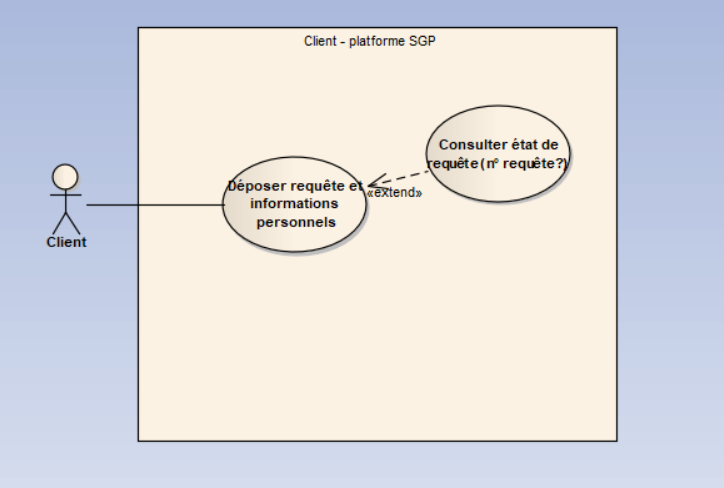
\includegraphics[width=0.92\textwidth]{Figures/GENERAL/Client.png}
    \caption{Cas d'utilisation — Client}
\end{figure}
\textbf{Client — description}
Le client dépose une requête avec ses informations, reçoit un accusé de réception et suit l'état d'avancement jusqu'à décision. Les données alimentent le référentiel et déclenchent la revue par la Direction.

\begin{figure}[H]
    \centering
    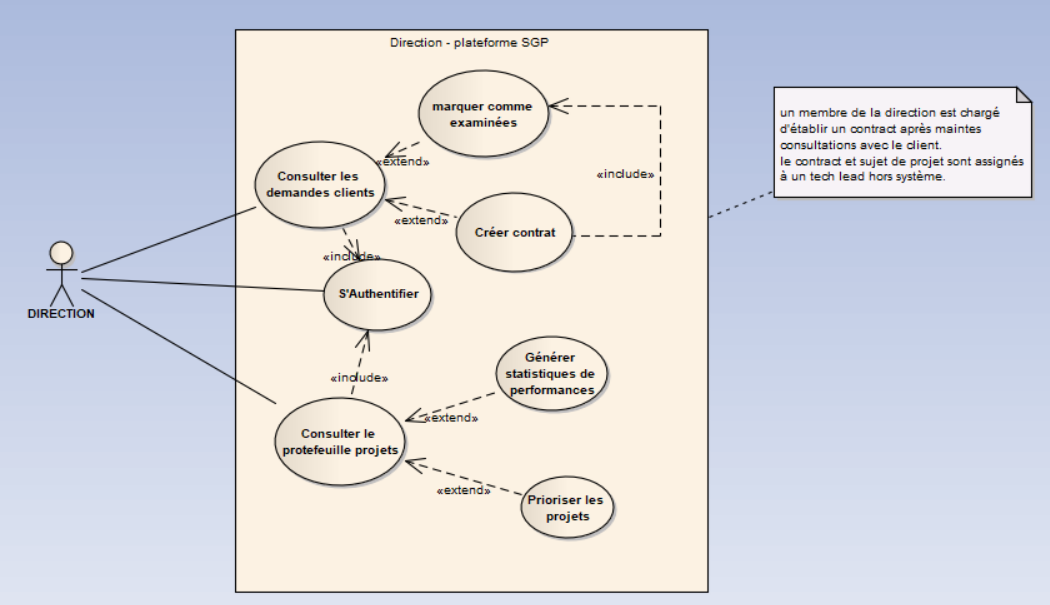
\includegraphics[width=0.92\textwidth]{Figures/GENERAL/Direction.png}
    \caption{Cas d'utilisation — Direction}
\end{figure}
\textbf{Direction — description}
La Direction consulte et marque les demandes, crée les contrats et priorise les projets en s'appuyant sur le portefeuille et les statistiques consolidées.

\begin{figure}[H]
    \centering
    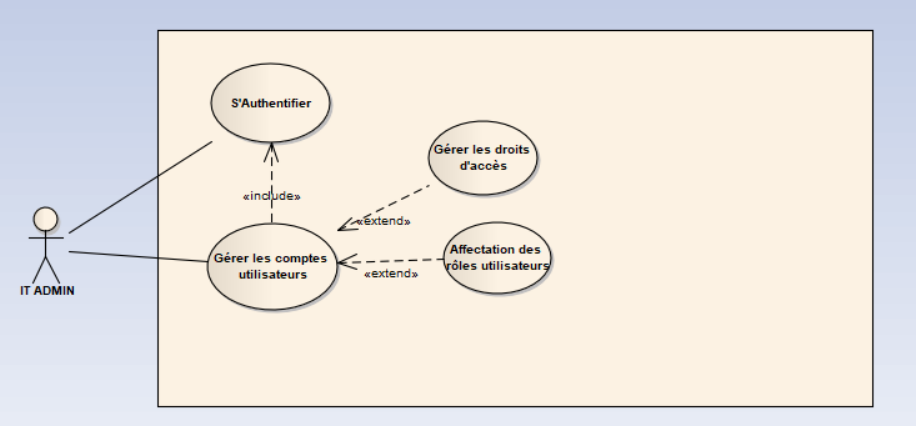
\includegraphics[width=0.92\textwidth]{Figures/GENERAL/ITADMIN.png}
    \caption{Cas d'utilisation — IT Admin}
\end{figure}
\textbf{IT Admin — description}
L'administrateur gère les comptes, les droits d'accès et l'affectation des rôles pour garantir un contrôle d'accès robuste.

\subsubsection*{Scrum}
\begin{figure}[H]
    \centering
    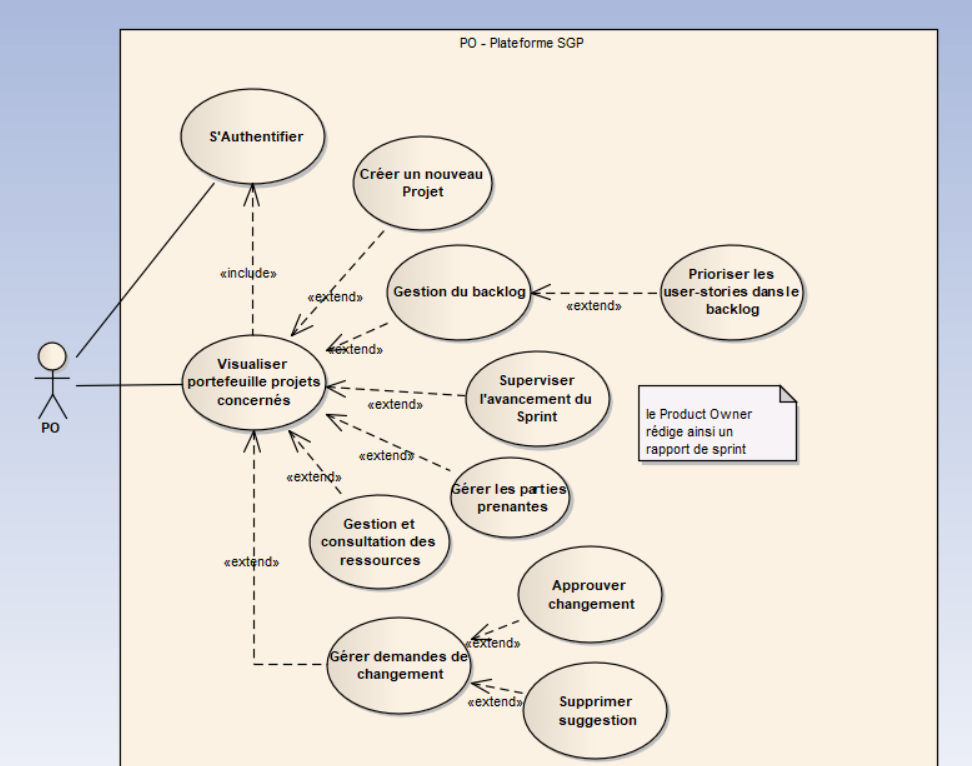
\includegraphics[width=0.92\textwidth]{Figures/SCRUM/PO.png}
    \caption{Cas d'utilisation — Product Owner}
\end{figure}
\textbf{PO — description}
Le PO ordonne le backlog, prépare la planification des sprints, valide les incréments et aligne vision, budget et jalons avec la Direction.

\begin{figure}[H]
    \centering
    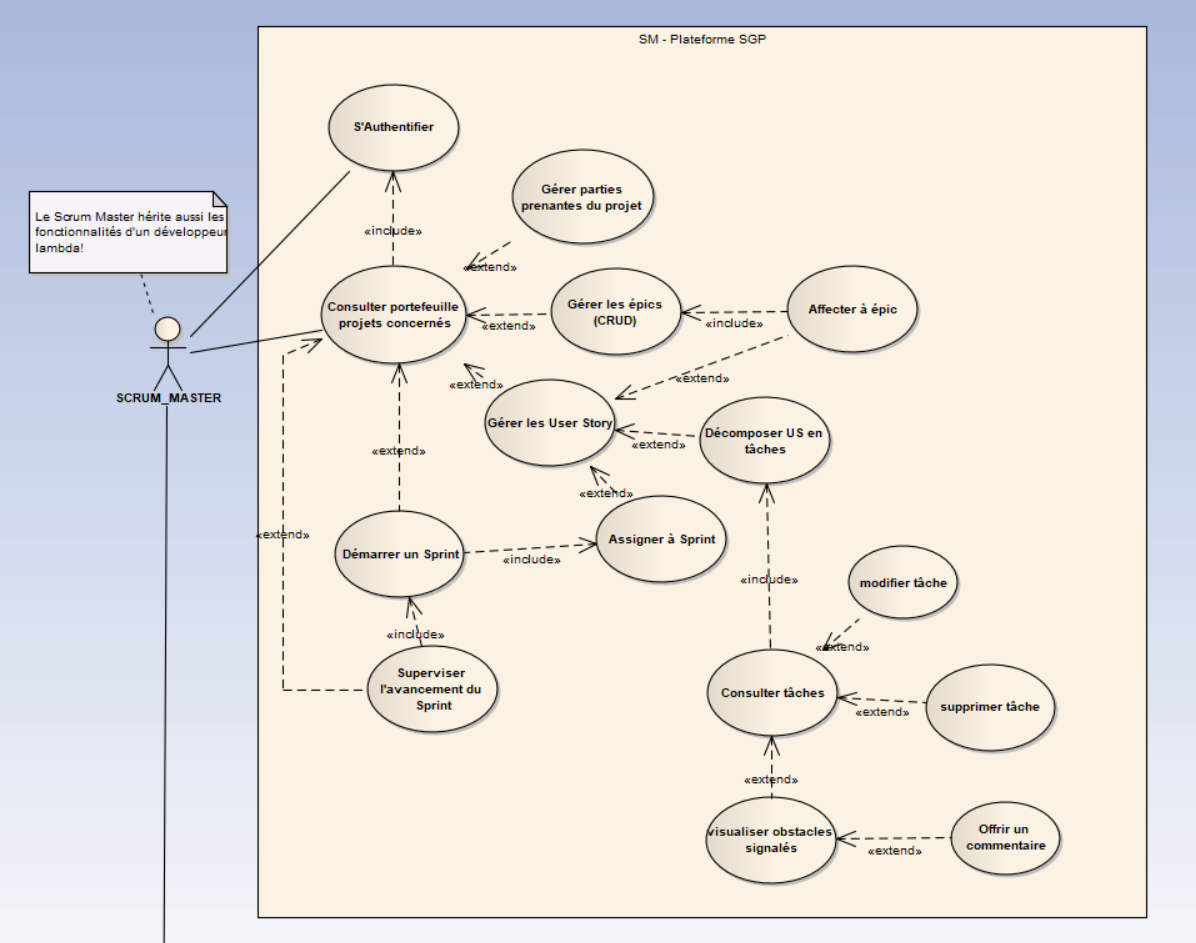
\includegraphics[width=0.92\textwidth]{Figures/SCRUM/SCRUMMASTER.png}
    \caption{Cas d'utilisation — Scrum Master}
\end{figure}
\textbf{Scrum Master — description}
Le SM facilite les rituels, retire les obstacles, suit burndown et vélocité, et coordonne les dépendances inter-équipes.

\begin{figure}[H]
    \centering
    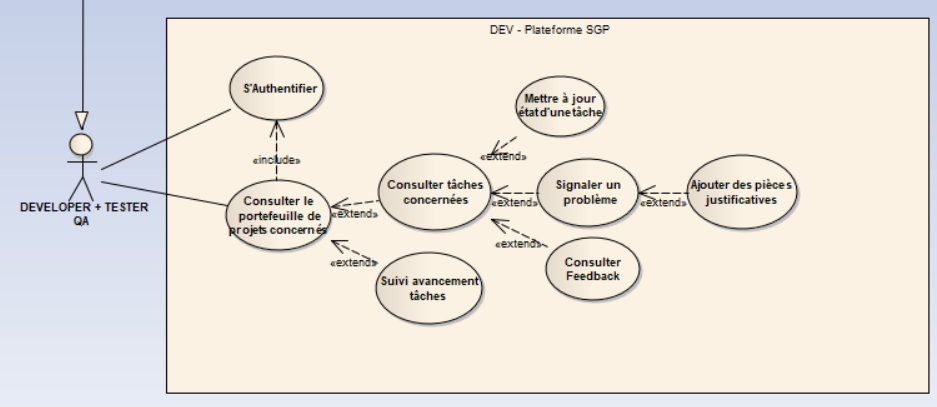
\includegraphics[width=0.92\textwidth]{Figures/SCRUM/DEVTESTERQA.png}
    \caption{Cas d'utilisation — Dev/Tester QA}
\end{figure}
\textbf{Dev/Tester QA — description}
Les membres de l'équipe mettent à jour les tâches, exécutent les tests et consignent le feedback et les pièces justificatives.

\subsubsection*{Itératif}
\begin{figure}[H]
    \centering
    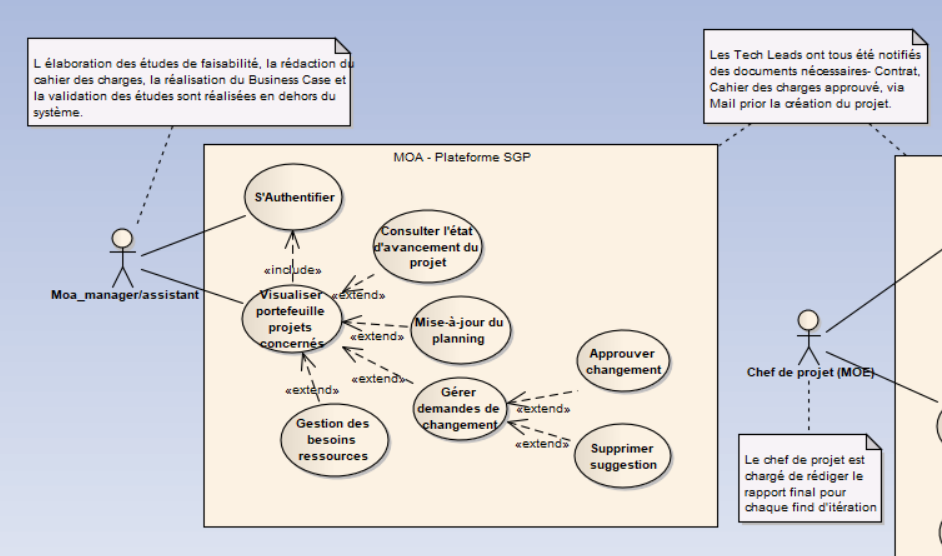
\includegraphics[width=0.92\textwidth]{Figures/ITERATIF/MOA.png}
    \caption{Cas d'utilisation — MOA}
\end{figure}
\textbf{MOA — description}
La MOA pilote la valeur, valide l'avancement et instruit/approuve les demandes de changement.

\begin{figure}[H]
    \centering
    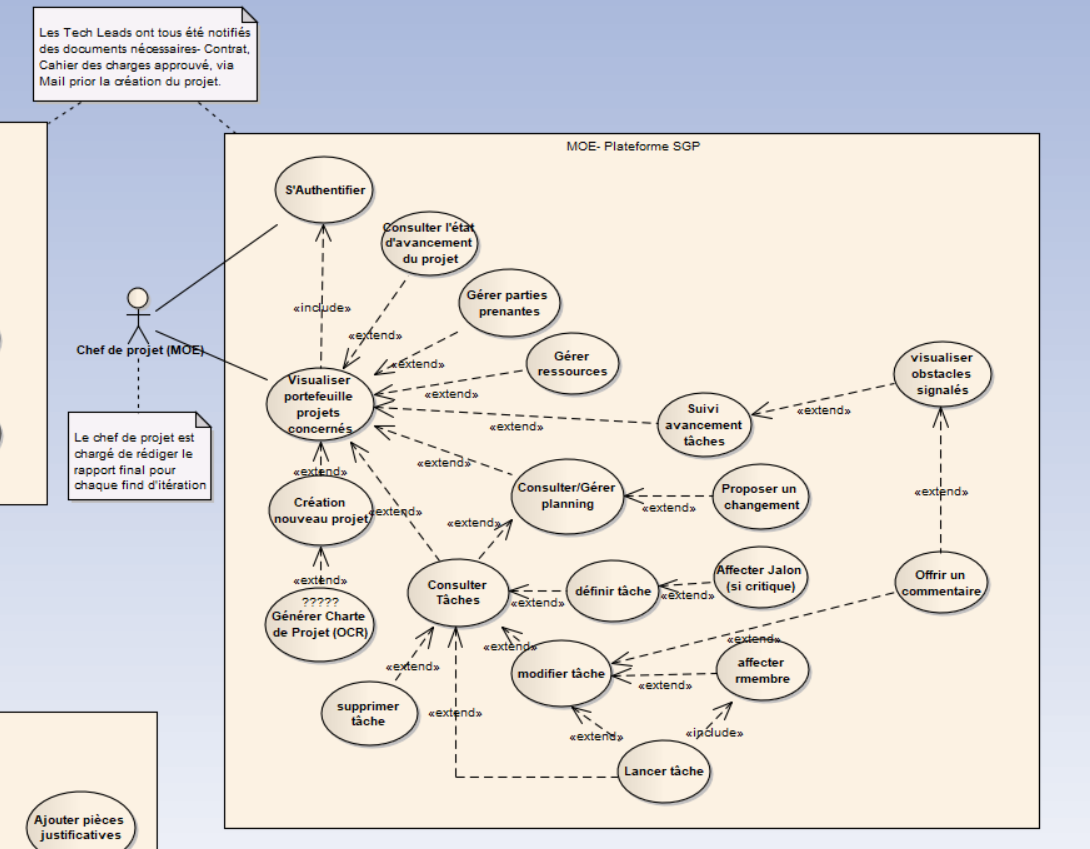
\includegraphics[width=0.92\textwidth]{Figures/ITERATIF/MOE.png}
    \caption{Cas d'utilisation — MOE}
\end{figure}
\textbf{MOE — description}
La MOE structure l'exécution, gère ressources et tâches, synchronise planning et jalons, et analyse l'impact des changements.

\begin{figure}[H]
    \centering
    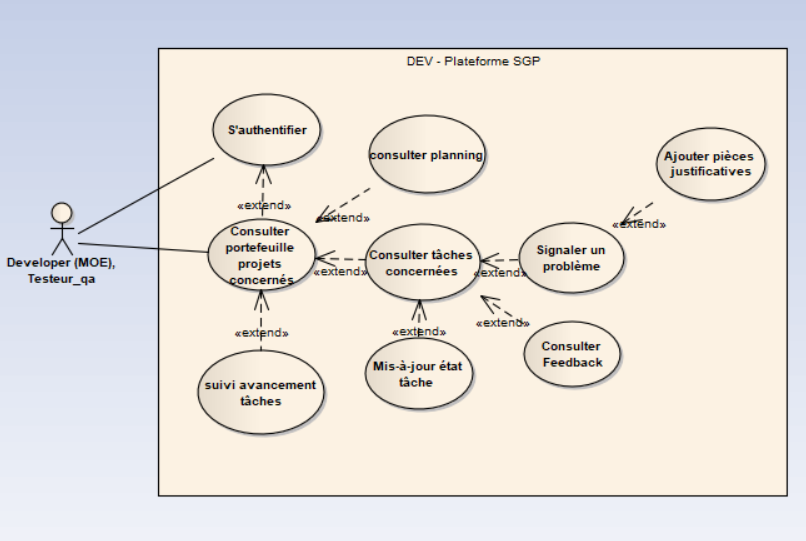
\includegraphics[width=0.92\textwidth]{Figures/ITERATIF/DEV.png}
    \caption{Cas d'utilisation — Dev (itératif)}
\end{figure}
\textbf{Dev (itératif) — description}
Le développeur met à jour l'état des tâches, signale les problèmes et fournit les éléments de preuve pour validation.

\subsection{Les diagrammes de séquence}

Cette section présente les flux d'interactions dynamiques entre les différents acteurs du système SGP selon deux méthodologies distinctes : Scrum et Itératif. Les diagrammes de séquence suivants décomposent chaque processus en étapes claires, montrant les échanges d'informations entre les acteurs humains et les composants système.

\subsubsection{Processus Scrum}

\begin{figure}[H]
    \centering
    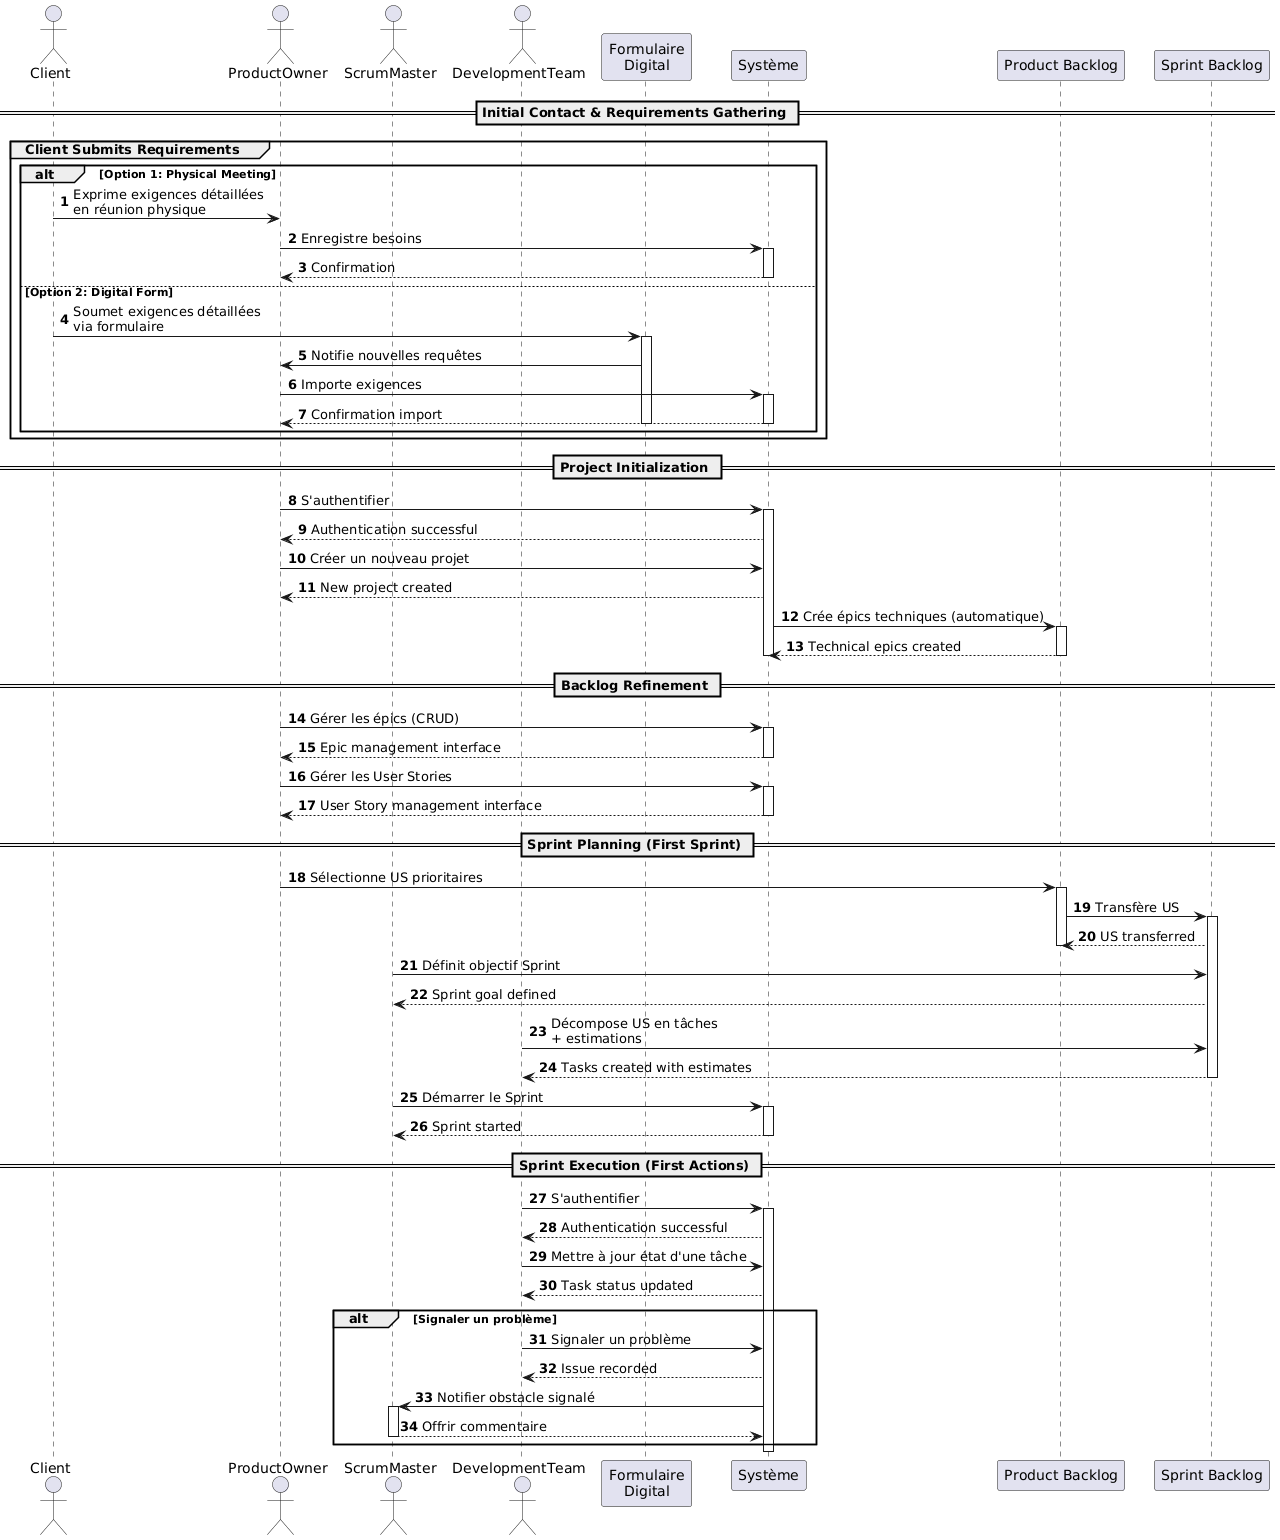
\includegraphics[width=\textwidth]{Figures/SCRUMseq.png}
    \caption{Diagramme de séquence : Processus Scrum}
    \label{fig:seq_scrum}
\end{figure}

\textbf{Processus Scrum (Figure \ref{fig:seq_scrum}) :} Ce diagramme illustre le cycle complet d'un projet Scrum, depuis la collecte des exigences jusqu'à l'exécution des premières actions de sprint. Le processus débute par la soumission des exigences du client, soit via une réunion physique avec le Product Owner, soit via un formulaire digital. Le Product Owner authentifie ensuite le système, crée un nouveau projet et gère les épics techniques automatiquement générés. La phase de raffinement du backlog permet au Product Owner de gérer les épics et les user stories. La planification du premier sprint implique la sélection des user stories prioritaires, leur transfert vers le sprint backlog, la définition de l'objectif du sprint par le Scrum Master, et la décomposition en tâches par l'équipe de développement. L'exécution du sprint commence par l'authentification de l'équipe, la mise à jour des statuts de tâches, et la possibilité de signaler des problèmes avec notification automatique au Scrum Master.

\subsubsection{Processus Itératif}

\begin{figure}[H]
    \centering
    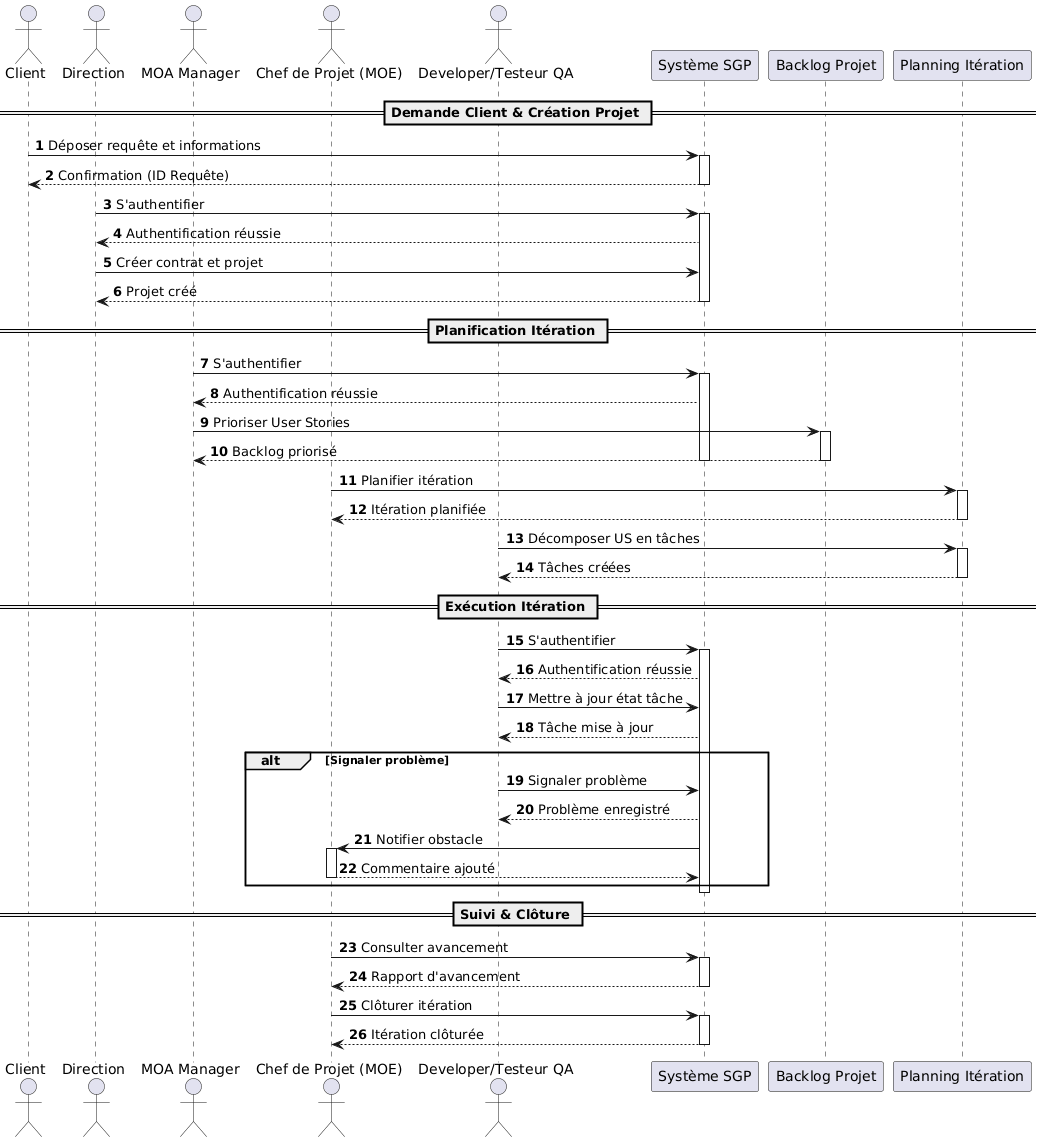
\includegraphics[width=\textwidth]{Figures/ITERATIFseq.png}
    \caption{Diagramme de séquence : Processus Itératif}
    \label{fig:seq_iteratif}
\end{figure}

\textbf{Processus Itératif (Figure \ref{fig:seq_iteratif}) :} Ce diagramme détaille le processus de gestion de projet itératif, structuré en quatre phases principales. La phase de \textbf{demande client et création de projet} commence par le dépôt d'une requête client avec informations détaillées, suivie de l'authentification de la Direction et de la création du contrat et du projet. La phase de \textbf{planification d'itération} implique l'authentification du MOA Manager, la priorisation des user stories dans le backlog projet, la planification de l'itération par le Chef de Projet (MOE), et la décomposition des user stories en tâches par l'équipe de développement. La phase d'\textbf{exécution d'itération} couvre l'authentification de l'équipe, la mise à jour des statuts de tâches, et la gestion des problèmes avec notification automatique au Chef de Projet. Enfin, la phase de \textbf{suivi et clôture} comprend la consultation de l'avancement par le MOA Manager et la clôture formelle de l'itération par le Chef de Projet.

\section{Modélisation du système}

Cette section présente les diagrammes de modélisation qui illustrent l'architecture et les interactions du système de gestion de projets.

\subsection{Contexte général}

\subsubsection{Situation actuelle et pratique existante}

Les activités projet étaient pilotées avec des outils épars (tableurs, e-mails) sans référentiel unique ni workflow tracé. L'absence de backlog consolidé, de sprints synchronisés et de suivi quotidien des tâches compliquait la planification, la coordination inter-rôles et la prise de décision.

\textbf{Lacunes identifiées dans l'ancien processus :}
\begin{itemize}
    \item \textbf{Fragmentation des outils :} Utilisation dispersée de tableurs Excel, e-mails et documents Word sans intégration, créant des silos d'information et des risques de perte de données.
    \item \textbf{Absence de traçabilité :} Impossibilité de suivre l'évolution d'une demande client jusqu'au livrable final, compliquant la justification des choix et la validation avec les clients.
    \item \textbf{Planification hétérogène :} Chaque équipe utilisait ses propres méthodes de planification des sprints et jalons, rendant impossible une vue d'ensemble cohérente du portefeuille.
    \item \textbf{Application inégale des rôles :} Les responsabilités des différents acteurs (PO, SM, Dev, etc.) n'étaient pas clairement définies ni respectées de manière uniforme.
    \item \textbf{Indicateurs insuffisants :} Manque d'indicateurs fiables sur l'avancement, la vélocité des équipes et la charge de travail, empêchant un pilotage efficace.
    \item \textbf{Notifications manuelles :} Absence d'automatisation des notifications, créant des retards dans la communication et les prises de décision.
    \item \textbf{Gestion des changements chaotique :} Aucun processus structuré pour analyser l'impact des changements sur les coûts, délais et ressources.
\end{itemize}

\subsubsection{Objectif de la solution}

L'objectif principal est de fournir une \textbf{SGP unifiée} qui centralise et standardise l'ensemble des processus de gestion de projets. Cette plateforme doit permettre la \textbf{capture structurée des demandes client} avec un workflow de validation par la Direction, incluant la collecte d'informations détaillées, l'évaluation de la faisabilité technique et commerciale, et la prise de décision éclairée sur l'opportunité de contractualiser.

La solution doit également supporter la \textbf{création et le paramétrage complet d'un projet}, incluant la définition des phases de développement, l'établissement des jalons de validation, l'allocation des ressources humaines et matérielles, et la configuration des règles métier spécifiques au projet.

L'\textbf{exécution Scrum} constitue le cœur de la plateforme, avec la gestion du backlog priorisé par le Product Owner, la planification et l'exécution des sprints par le Scrum Master, la décomposition en user stories détaillées, et le suivi des tâches opérationnelles par les équipes de développement.

\subsection{Enjeux et objectifs}

Les enjeux majeurs du \textbf{SGP} sont: \textbf{visibilité portefeuille}, \textbf{pilotage par la valeur}, \textbf{réduction du temps de cycle} et \textbf{maîtrise des risques et des changements}. Ces enjeux se traduisent par les objectifs concrets suivants:

\begin{itemize}
    \item \textbf{Centralisation des artefacts} du projet: \texttt{Projet, Phase, Sprint, UserStory, Tache, Jalon, Backlog, Livrable, Validation, Changement}.
    \item \textbf{Exécution agile outillée}: priorisation du backlog par le PO, planification/démarrage de sprints par le SM, tableaux Kanban et mises à jour de tâches par Dev/QA.
    \item \textbf{Gouvernance et conformité}: jalons, validations de livrables, gestion des changements avec traçabilité.
    \item \textbf{Rôles et accès} robustes (JWT/OAuth2 Microsoft), gardes côté Angular et contrôles côté Spring Security.
    \item \textbf{Indicateurs temps réel}: KPI par projet/sprint (vélocité, avancement, charge, qualité), notifications WebSocket, analytics et exports via Power BI.
    \item \textbf{Référentiel amont}: intégration des demandes clients (\texttt{ClientInquiry}) et des contrats, menant à la création de projets.
\end{itemize}

\subsection{Méthodologie adoptée}

Pour ce projet, nous avons opté pour la \textbf{méthodologie Scrum}, qui favorise un développement itératif et incrémental à travers des sprints. Chaque sprint est planifié sur une durée de deux semaines, permettant de livrer des fonctionnalités prêtes à l'usage tout en recueillant régulièrement des retours des parties prenantes.

\subsubsection{Le cycle de vie du projet}

Le cycle de vie de notre projet comprend les activités suivantes :

\begin{enumerate}
    \item \textbf{Analyse des besoins et faisabilité :} Identification, recueil et formalisation des besoins fonctionnels et non fonctionnels, ainsi que des contraintes techniques et organisationnelles.
    \item \textbf{Planification et priorisation :} Création du backlog produit, définition des priorités et planification des tâches pour chaque sprint.
    \item \textbf{Conception :} Élaboration des spécifications générales et détaillées de l'architecture logicielle, des bases de données et des interfaces utilisateur.
    \item \textbf{Développement :} Implémentation progressive des fonctionnalités prévues dans les sprints, avec des revues de code et une intégration continue.
    \item \textbf{Tests :} Vérification de chaque fonctionnalité par des tests unitaires, fonctionnels et d'intégration pour garantir leur conformité aux spécifications.
    \item \textbf{Documentation :} Rédaction des informations nécessaires à l'utilisation, la maintenance et les futures évolutions du logiciel.
    \item \textbf{Livraison et déploiement :} Livraison progressive des incréments et mise en production du produit final.
\end{enumerate}

Cette approche agile assure une meilleure collaboration entre les parties prenantes et une flexibilité accrue face aux changements, tout en maintenant un haut niveau de qualité.

% --- Image de la méthodologie SCRUM ---
\begin{figure}[H] 
    \centering
    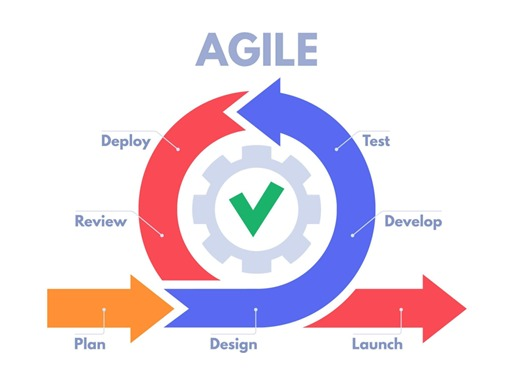
\includegraphics[width=1\textwidth]{Figures/Model_SCRUM.jpg}
    \caption{Modèle de la méthodologie SCRUM}
    \label{fig:methodo_scrum}
\end{figure}

\subsubsection{Modèle de travail}

Un projet logiciel doit suivre différentes phases jalonnées par des points de contrôle clés afin de garantir sa gestion dans un contexte de qualité. Chaque étape est associée à des livrables spécifiques validés en fonction des objectifs définis. Cette approche permet de maîtriser la conformité des livrables aux besoins exprimés, tout en s'assurant du respect des contraintes de coûts et de délais.

Parmi les modèles de développement logiciel, nous avons adopté une approche itérative basée sur la méthodologie Scrum. Contrairement au modèle en cascade, cette méthode repose sur des cycles itératifs (sprints) qui favorisent l'adaptation continue aux besoins évolutifs du projet. Chaque sprint se termine par la production d'un incrément fonctionnel validé par les parties prenantes.

% --- Image du modèle AGILE ---
\begin{figure}[H] 
    \centering
    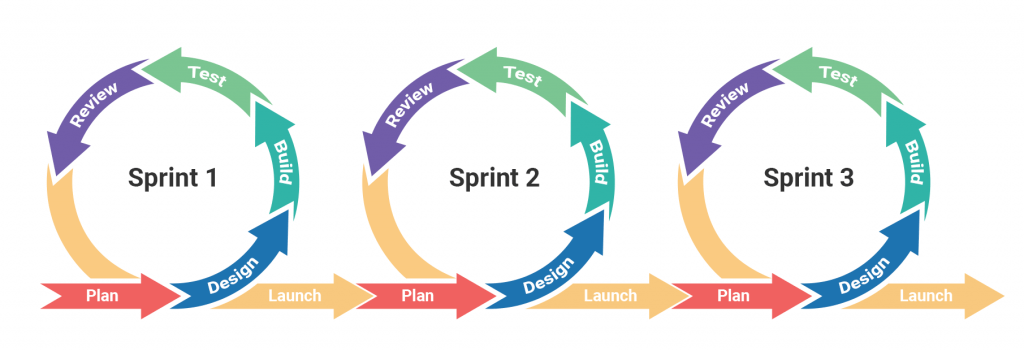
\includegraphics[width=0.8\textwidth]{Figures/agile.png}
    \caption{Modèle de la méthodologie AGILE}
    \label{fig:methodo_agile}
\end{figure}

\subsection{Planification du projet}

\subsubsection{Étapes clés}

La planification est une étape clé qui consiste à organiser et prioriser les tâches du projet, à estimer les ressources nécessaires et à identifier les profils requis pour chaque phase. Elle permet également de définir un calendrier réaliste et de répartir les responsabilités au sein de l'équipe. Conformément à la méthodologie adoptée et au contexte de notre projet, nous avons structuré le travail en sprints successifs, chacun ayant des objectifs précis, afin de garantir une livraison itérative, flexible et facilement ajustable en fonction des retours et imprévus.

\begin{itemize}
    \item \textbf{Sprint 0 : Compréhension du projet} \\
    Analyse des besoins et création du backlog produit en priorisant les fonctionnalités de la plateforme de gestion de projets.
    \item \textbf{Sprint 1 : Conception et spécifications techniques} \\
    Modélisation UML (cas d'utilisation, séquences, classes) et définition de l'architecture du système et des interfaces.
    \item \textbf{Sprint 2 : Gestion du paramétrage} \\
    Développement des fonctionnalités de gestion des utilisateurs et des rôles projet.
    \item \textbf{Sprint 3 : Gestion des activités} \\
    Implémentation des modules pour la gestion des projets, sprints, user stories, et tâches.
    \item \textbf{Sprint 4 : Gestion des statistiques} \\
    Création des tableaux de bord et rapports : KPI de projets, vélocité des équipes, burndown charts, et analytics Power BI.
    \item \textbf{Sprint 5 : Tests, validation et déploiement} \\
    Réalisation des tests fonctionnels et d'intégration, correction des anomalies, validation avec les utilisateurs, et déploiement en production.
\end{itemize}

L'approche agile a permis une gestion flexible et réactive, assurant une livraison progressive et cohérente du système. Elle a favorisé une meilleure adaptation aux changements et aux contraintes rencontrées en cours de projet. Grâce aux retours réguliers des utilisateurs, il a été possible d'ajuster les priorités et d'orienter les développements vers les besoins réels. En remplaçant les outils traditionnels comme les diagrammes de Gantt par la planification par sprints, la collaboration au sein de l'équipe a été renforcée, l'efficacité globale améliorée et la visibilité sur l'avancement du projet nettement optimisée.

\subsubsection{Calendrier prévisionnel et jalons principaux}

% ---- TABLEAU DE PLANIFICATION DES SPRINTS ----

\begingroup
\footnotesize
\setlength{\tabcolsep}{4pt}
\setlength{\LTpre}{12pt}

\begin{longtable}{|p{1.2cm}|p{2.8cm}|p{4.8cm}|p{1.2cm}|p{1.2cm}|p{1.8cm}|p{1.8cm}|}

    \endfirsthead

    \hline
    \textbf{Sprint} & \textbf{TITRE} & \textbf{TÂCHES} & \parbox[t]{1.3cm}{\centering\bfseries PRIO-RITÉ} & \textbf{ÉTAT} & \parbox[t]{1.8cm}{\centering\bfseries DATE DE\\DÉBUT} & \parbox[t]{1.8cm}{\centering\bfseries DATE DE\\FIN} \\
    \hline
    \endhead

\endfoot

    % === CORPS DU TABLEAU (MIS À JOUR POUR LE SYSTÈME DE GESTION DE PROJETS) ===
     % Sprint 00
\multirow{1}{=}{\centering\textbf{Sprint 00}} & \multirow{1}{=}{\centering Étude préliminaire} & Analyse des besoins et création du backlog produit & High & Complete & 01/07/2025 & 06/07/2025 \\ \hline
    % Sprint 01
    \multirow{6}{=}{\centering\textbf{Sprint 01}} & \multirow{6}{=}{\centering Analyse et Conception} & Création des maquettes UI/UX & High & Complete & 07/07/2025 & 10/07/2025 \\ \cline{3-7}
    & & Rédaction du cahier des charges & Normal & Complete & 11/07/2025 & 13/07/2025 \\ \cline{3-7}
    & & Élaboration du diagramme de cas d'utilisation & High & Complete & 14/07/2025 & 16/07/2025 \\ \cline{3-7}
    & & Modélisation du diagramme de classes & Normal & Complete & 17/07/2025 & 19/07/2025 \\ \cline{3-7}
    & & Conception du diagramme de séquence & High & Complete & 20/07/2025 & 22/07/2025 \\ \cline{3-7}
    & & Rédaction du dossier de conception & High & Complete & 23/07/2025 & 25/07/2025 \\ \hline

    % Sprint 02
    \multirow{3}{=}{\centering\textbf{Sprint 02}} & \multirow{3}{=}{\centering Gestion des Utilisateurs} & Développement de l'authentification et autorisation & High & Complete & 26/07/2025 & 28/07/2025 \\ \cline{3-7}
    & & Gestion des rôles et permissions & High & Complete & 29/07/2025 & 31/07/2025 \\ \cline{3-7}
    & & Interface de gestion des utilisateurs & Normal & Complete & 01/08/2025 & 02/08/2025 \\ \hline

    % Sprint 03
    \multirow{4}{=}{\centering\textbf{Sprint 03}} & \multirow{4}{=}{\centering Gestion des Projets} & Création et gestion des projets & High & Complete & 03/08/2025 & 05/08/2025 \\ \cline{3-7}
    & & Gestion des sprints et user stories & High & Complete & 06/08/2025 & 08/08/2025 \\ \cline{3-7}
    & & Système de tâches et Kanban board & High & Complete & 09/08/2025 & 11/08/2025 \\ \cline{3-7}
    & & Gestion des jalons et phases & Normal & Complete & 12/08/2025 & 14/08/2025 \\ \hline

    % Sprint 04
    \multirow{3}{=}{\centering\textbf{Sprint 04}} & \multirow{3}{=}{\centering Tableaux de Bord} & Dashboard principal avec KPI & High & Complete & 15/08/2025 & 16/08/2025 \\ \cline{3-7}
    & & Rapports de vélocité et burndown charts & Normal & Complete & 17/08/2025 & 18/08/2025 \\ \cline{3-7}
    & & Intégration Power BI et analytics & Normal & Complete & 19/08/2025 & 20/08/2025 \\ \hline

    % Sprint 05
    \multirow{2}{=}{\centering\textbf{Sprint 05}} & \multirow{2}{=}{\centering Tests et Livraison} & Tests fonctionnels et vérifications d'intégration & High & Complete & 21/08/2025 & 22/08/2025 \\ \cline{3-7}
& & Livraison finale de la plateforme & Normal & Complete & 23/08/2025 & 25/08/2025 \\ \hline

\caption{Planning des Sprints}
\label{tab:planning_sprints}
\endlastfoot

\end{longtable}
\endgroup

\section{Conclusion}

Ce chapitre a présenté la modélisation et l'implémentation de notre solution de gestion de projets. Nous avons détaillé les blocs fonctionnels qui constituent le cœur de la plateforme, couvrant l'ensemble du cycle de vie d'un projet depuis la gestion des utilisateurs jusqu'aux analytics avancés. 

La méthodologie Scrum adoptée, avec son cycle de vie structuré en sept étapes clés et son organisation en sprints successifs, garantit une flexibilité et une adaptabilité optimales face aux évolutions des besoins. Cette approche agile maintient un haut niveau de qualité et assure une collaboration efficace entre toutes les parties prenantes du projet.

La définition détaillée des blocs fonctionnels et des règles de gestion garantit une implémentation cohérente et robuste de la plateforme. Chaque module répond à des besoins métier spécifiques tout en s'intégrant harmonieusement dans l'écosystème global de la SGP. Cette approche modulaire facilite la maintenance, l'évolution et l'adaptation de la solution aux besoins changeants de l'organisation.
